\documentclass{beamer}

\mode<presentation> {

% The Beamer class comes with a number of default slide themes
% which change the colors and layouts of slides. Below this is a list
% of all the themes, uncomment each in turn to see what they look like.

%\usetheme{default}
%\usetheme{AnnArbor}
%\usetheme{Antibes}
%\usetheme{Bergen}
%\usetheme{Berkeley}
%\usetheme{Berlin}
%\usetheme{Boadilla}
%\usetheme{CambridgeUS}
%\usetheme{Copenhagen}
%\usetheme{Darmstadt}
%\usetheme{Dresden}
\usetheme{Frankfurt}
%\usetheme{Goettingen}
%\usetheme{Hannover}
%\usetheme{Ilmenau}
%\usetheme{JuanLesPins}
%\usetheme{Luebeck}
%\usetheme{Madrid}
%\usetheme{Malmoe}
%\usetheme{Marburg}
%\usetheme{Montpellier}
%\usetheme{PaloAlto}
%\usetheme{Pittsburgh}
%\usetheme{Rochester}
%\usetheme{Singapore}
%\usetheme{Szeged}
%\usetheme{Warsaw}

% As well as themes, the Beamer class has a number of color themes
% for any slide theme. Uncomment each of these in turn to see how it
% changes the colors of your current slide theme.

%\usecolortheme{albatross}
%\usecolortheme{beaver}
%\usecolortheme{beetle}
\usecolortheme{crane}
%\usecolortheme{dolphin}
%\usecolortheme{dove}
%\usecolortheme{fly}
%\usecolortheme{lily}
%\usecolortheme{orchid}
%\usecolortheme{rose}
%\usecolortheme{seagull}
%\usecolortheme{seahorse}
%\usecolortheme{whale}
%\usecolortheme{wolverine}

%\setbeamertemplate{footline} % To remove the footer line in all slides uncomment this line
%\setbeamertemplate{footline}[page number] % To replace the footer line in all slides with a simple slide count uncomment this line

%\setbeamertemplate{navigation symbols}{} % To remove the navigation symbols from the bottom of all slides uncomment this line
}

\usepackage{extpfeil}
\usepackage{extarrows} %Allows long equation signs
\usepackage{graphicx} % Allows including images
\usepackage{booktabs} % Allows the use of \toprule, \midrule and \bottomrule in tables
\usepackage{physics}
\usepackage{tikz}
\usepackage{cite}
%花体字母
\usepackage{amsthm,amsmath,amssymb}
\usepackage{mathrsfs}
\usepackage{dutchcal}
\usepackage{circuitikz}
\usepackage{multirow}

%----------------------------------------------------------------------------------------
%	TITLE PAGE
%----------------------------------------------------------------------------------------

\title[VP260 RC]{Final Review} % The short title appears at the bottom of every slide, the full title is only on the title page

\author{VP260 TA Group} % Your name
\institute[UM-SJTU JI] % Your institution as it will appear on the bottom of every slide, may be shorthand to save space
{
    University of Michigan - Shanghai Jiao Tong University Joint Institute\\% Your institution for the title page
\medskip
}
\date{\today} % Date, can be changed to a custom date

\AtBeginSection[]
{
  \begin{frame}
    \frametitle{Table of Contents}
    \tableofcontents[currentsection]
  \end{frame}
}

\begin{document}

\begin{frame}
    \titlepage % Print the title page as the first slide
\end{frame}

\begin{frame}{Outline}
    \tableofcontents
\end{frame}

%----------------------------------------------------------------------------------------
%	 SECTION 1
%----------------------------------------------------------------------------------------
\section{Fundamental Concepts}

\subsection{Maxwell's Equation} % Section title slide, unnumbered

\begin{frame}{Faraday’s Law and Lenz' Law}
    A changing magnetic field induces an electric field.

    \begin{block}{Faraday's law}
        \begin{equation}
            \oint \va{E} \vdot \dd{\va{l}} = -\oint \pdv{\va{B}}{t} \dd{\va{a}}
        \end{equation}

        \begin{equation}
            \curl{\va{E}} = -\pdv{\va{B}}{t}
        \end{equation}
    \end{block}

    \begin{block}{Lenz' law}
        The negative sign means that nature abhors a change in flux.
    \end{block}
\end{frame}

\begin{frame}{Displacement Current}
    A changing electric field induces a magnetic field.

    \begin{columns}
        \begin{column}{0.5\textwidth}
            \begin{figure}[htbp]
                \centering
                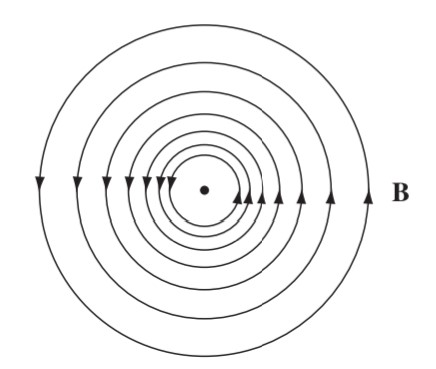
\includegraphics[width=\textwidth]{Images/amp.jpg}
            \end{figure}
        \end{column}
        \begin{column}{0.5\textwidth}
            \begin{block}{Displacement current}
                \begin{equation}
                    \va{J}_d = \epsilon_0 \pdv{\va{E}}{t}
                \end{equation}
            \end{block}
        \end{column}
    \end{columns}
\end{frame}

\begin{frame}{Maxwell's Equation}
    \begin{table}[htbp]
        \centering
        \begin{tabular}{ll}
            \toprule
            Integral Form                                                                         & Differential Form                                              \\
            \midrule
            $\oint \va{E}\vdot\dd{\va{a}}=\frac{Q_{\text{enc}}}{\epsilon_0}$                      & $\div{\va{E}} = \frac{\rho}{\epsilon_0}$                       \\ \addlinespace
            $\oint \va{E}\vdot\dd{\va{l}}= -\dv{\Phi_B}{t}$                                       & $\curl{\va{E}}=-\pdv{\va{B}}{t}$                               \\ \addlinespace
            $\oint \va{B}\vdot\dd{\va{a}}=0$                                                      & $\div{\va{B}} = 0$                                             \\ \addlinespace
            $\oint \va{B}\vdot\dd{\va{l}}=\mu_0 I_{\text{enc}} + \mu_0 \epsilon_0 \dv{\Phi_E}{t}$ & $\curl{\va{B}}=\mu_0 \va{J}+ \mu_0 \epsilon_0 \pdv{\va{E}}{t}$ \\
            \bottomrule
        \end{tabular}
    \end{table}
\end{frame}

\subsection{Magnetic Vector Potential}

\begin{frame}{Scalar and Vector Potentials}
    \begin{block}{Vector Potential}
        \begin{equation}
            \va{B} = \curl \va{A}
        \end{equation}
        \begin{equation}
            \va{E} = -\grad V - \pdv{\va{A}}{t}
        \end{equation}
    \end{block}

    \begin{block}{Gauge Transform}
        \begin{equation}
            \va{A}'=\va{A}+\nabla \lambda
        \end{equation}
        \begin{equation}
            V'=V-\frac{\partial \lambda}{\partial t}
        \end{equation}
    \end{block}
\end{frame}

\begin{frame}{Gauge}
    \begin{block}{Coulomb Gauge}
        \begin{equation*}
            \div\va{A} = 0
        \end{equation*}
    \end{block}

    \begin{block}{Lorenz Gauge}
        \begin{equation*}
            \div \va{A} = -\mu_0\epsilon_0\pdv{V}{t}
        \end{equation*}
    \end{block}

    \begin{block}{Landau Gauge}
        For uniform magnetic field $\va{B} = B \vu{z}$,
        \begin{equation*}
            \va{A} = By \vu{x}
        \end{equation*}
    \end{block}
\end{frame}

\subsection{Inductance}

\begin{frame}{Inductance (unit: H)}
    \begin{block}{Mutual Inductance}
        \begin{equation}
            M_{21}=\frac{\mu_{0}}{4 \pi} \oint \oint \frac{d \mathbf{l}_{1} \cdot d \mathbf{l}_{2}}{r}
        \end{equation}
        \begin{equation}
            M_{21} = M_{12}
        \end{equation}
    \end{block}

    \begin{block}{Self Inductance}
        \begin{equation}
            \Phi = L I
        \end{equation}
        \begin{equation}
            \varepsilon = - L \dv*{I}{t}
        \end{equation}

        Pay attention to the direction (potential drop through inductor).
    \end{block}

    \begin{itemize}
        \item Inductor: $W_L = \frac{1}{2} L I^2$
        \item Magnetic field energy density: $u = \frac{B^2}{2 \mu_r\mu_0}$
    \end{itemize}
\end{frame}

\subsection{Circuits}

\begin{frame}{RL, LC, RLC Circuits}
    \begin{table}[htbp]
        \centering
        \begin{tabular}{l c l}
            \toprule
            RC                   & $i(t)=\epsilon/R(1-exp(-t/\tau))$                                                                 & $\tau=RC$               \\ \addlinespace[1em]
            RL                   & $i(t)=\epsilon/R(1-exp(-t/\tau))$                                                                 & $\tau=L/R$              \\ \addlinespace[1em]
            LC                   & $q(t) = A\sin(\omega_0 t) + B\cos(\omega_0 t)$                                                    & $\omega_0 = 1\sqrt{LC}$ \\ \addlinespace[1em]
            \multirow{3}{*}{RLC} & \multirow{3}{*}{$\frac{d^{2} I(t)}{d t^{2}}+\frac{R}{L} \frac{d I(t)}{d t}+\frac{1}{L C} I(t)=0$} & Underdamped             \\
                                 &                                                                                                   & Critical damping        \\
                                 &                                                                                                   & Overdamped              \\
            \bottomrule
        \end{tabular}
    \end{table}
\end{frame}


\begin{frame}{AC Circuit}
    \begin{block}{AC current}
        \begin{equation}
            i(t) = I_0 \cos(\omega t + \phi)
        \end{equation}
        \begin{equation}
            i(t) = \Re{I_0 e^{\phi j} e^{j\omega t}}
        \end{equation}
    \end{block}
    \begin{itemize}
        \item Rectified average current: $I_{rav} = \frac{1}{T}\int_{t_1}^{t_1+T}\abs{i(t)}\dd t = \frac{2}{\pi}I$
        \item Root-mean-square current: $I_{rms} = \sqrt{\frac{1}{T}\int_{t_1}^{t_1+T}i^2(t)\dd t} = \frac{I}{\sqrt{2}}$
    \end{itemize}
\end{frame}

\begin{frame}{Elements in AC}
    \begin{table}[htbp]
        \centering
        \begin{tabular}{l c c}
            \toprule
            Elements & Impedance        & Phase    \\
            \midrule
            R        & $R$              & 0        \\
            L        & $j\omega L $     & $\pi/2$  \\
            C        & $1/(j \omega C)$ & $-\pi/2$ \\
            \bottomrule
        \end{tabular}
    \end{table}

    \begin{block}{Resonance}
        \begin{equation}
            \abs{Z} = \sqrt{R^2+(\omega L - \frac{1}{\omega C})^2 }
        \end{equation}
        Resonance happens when $\omega_0 = \frac{1}{LC}$
    \end{block}

    \begin{block}{ Power}
        \begin{equation}
            \overline{P} = V_{rms} I_{rms}
        \end{equation}
    \end{block}
\end{frame}

\subsection{Electromagnetic waves}

\begin{frame}{Classical Wave Equation}
    \begin{block}{Classical wave equation}
        \begin{equation}
            \pdv[2]{f}{x} = \frac{1}{v^2} \pdv[2]{f}{t}
        \end{equation}
    \end{block}
    \vfill
    \begin{itemize}
        \item $f$ is displacement, $v$ is speed of propagation;
        \item Example: sound, wave on a string;
        \item Solution: $f(x, t) = g(x - vt) + h(x + vt)$.
    \end{itemize}
\end{frame}

\begin{frame}{Sinusoidal Waves}
    \begin{block}{Sinusoidal wave}
        \begin{equation}
            f(x, t) = A \cos(k (x - vt) + \varphi)
        \end{equation}
    \end{block}

    \begin{block}{Complex wave function}
        \begin{equation}
            \tilde{f}(x, t) = \tilde{A} e^{i(kx-\omega t)}
        \end{equation}
    \end{block}

    \begin{table}[htbp]
        \centering
        %\caption{name}
        \begin{tabular}{ll}
            $A$                        & amplitude                                 \\
            $k$                        & wave number                               \\
            $k(x-vt)+\varphi$          & phase                                     \\
            $\varphi$                  & phase constant ($0 \leq \varphi < 2 \pi$) \\
            $\lambda = \frac{k}{2\pi}$ & wave length                               \\
            $T = \frac{2\pi}{kv}$      & period                                    \\
            $\nu = \frac{1}{T}$        & frequency                                 \\
            $\omega = 2\pi \nu$        & angular frequency                         \\
        \end{tabular}
    \end{table}

\end{frame}


\begin{frame}{Electromagnetic Waves in Vacuum}
    \begin{block}{Electromagnetic waves in vacuum}
        \begin{equation}
            \va{E}(z, t) = E_0 \cos(kz - \omega t + \varphi) \vu{x},
        \end{equation}
        \begin{equation}
            \va{B}(z, t) = \frac{1}{c}E_0 \cos(kz - \omega t + \varphi) \vu{y}.
        \end{equation}
    \end{block}
    \begin{itemize}
        \item Transverse wave;
        \item Two field are in phase and perpendicular;
        \item The direction of polarization is the same as $\va{E}$.
        \item $\tilde{\vb{B}}_0 = \frac{k}{\omega} \left(\vu{z} \times \tilde{\vb{E}}_0 \right) = \frac{1}{c} \left(\vu{z} \times \tilde{\vb{E}}_0 \right)$
    \end{itemize}

    \begin{figure}[htbp]
        \centering
        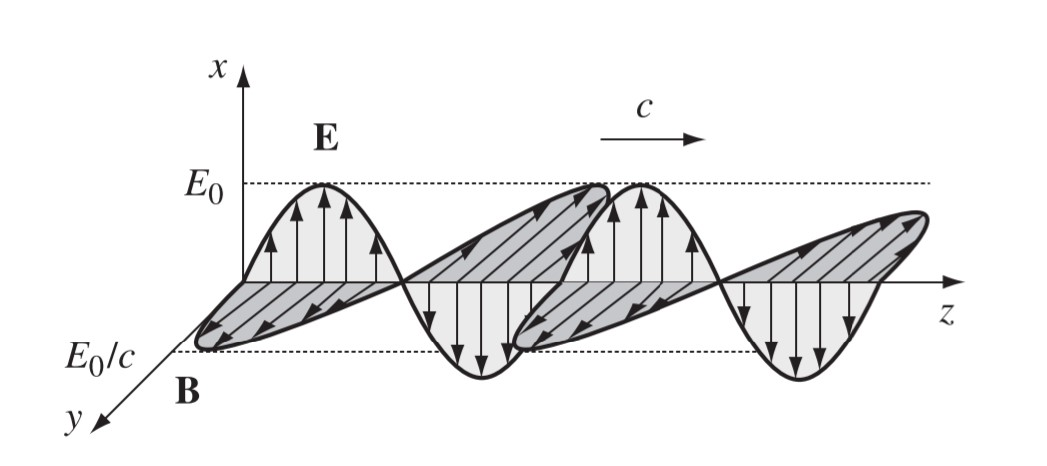
\includegraphics[width=0.5\textwidth]{Images/emwave.jpg}
    \end{figure}
\end{frame}

\begin{frame}{Poynting Vector}
    We define the energy flux (energy per unit area, per unit time) as Poynting vector,

    \begin{block}{Poynting Vector}
        \begin{equation}
            \va{S} = \frac{1}{\mu_0} (\va{E} \times \va{B})
        \end{equation}
    \end{block}

    For the sinusoidal waves, $\va{S} = cu \vu{z}$ where $u = \epsilon_0 E^2$ is energy density.
\end{frame}

\subsection{Optics}

\begin{frame}{Reflection and Refraction}
    \begin{columns}
        \begin{column}{.3\linewidth}
            \begin{figure}[htbp]
                \centering
                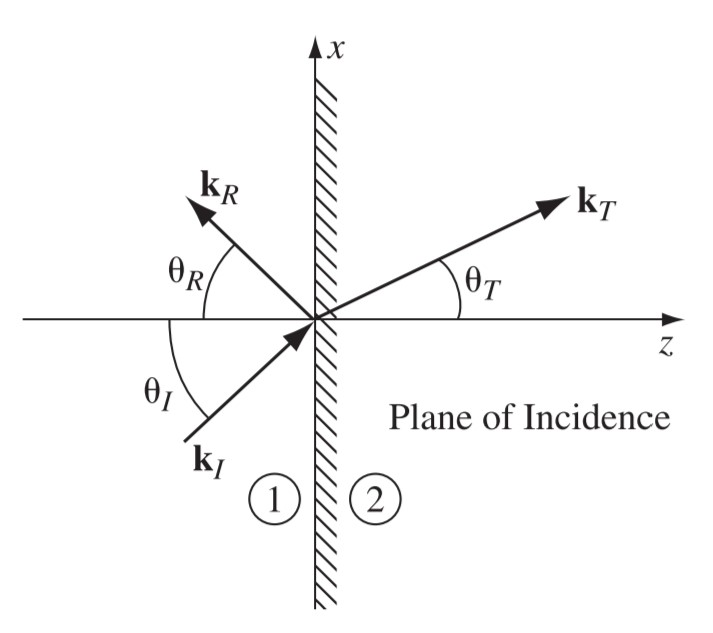
\includegraphics[width=\textwidth]{Images/re.jpg}
            \end{figure}
        \end{column}
        \begin{column}{.7\linewidth}
            \begin{block}{Law of reflection}
                \begin{equation}
                    \theta_I = \theta_R
                \end{equation}
            \end{block}

            \begin{block}{Law of refraction (Snell's law)}
                \begin{equation}
                    \frac{\sin \theta_T}{\sin \theta_I} = \frac{n_1}{n_2}
                \end{equation}
            \end{block}
            \begin{itemize}
                \item $n_i = v_i / c$ is called refractive index.
                \item When $\theta_I > \theta_{cr}$, where $\sin \theta_{cr} = n_2 / n_1$, there is a total internal reflection.
            \end{itemize}
        \end{column}
    \end{columns}
\end{frame}

\begin{frame}{Huygens' Principle}
    \begin{block}{Huygens' principle}
        Every point of the wavefront may be considered as a source of secondary wavelets that propagate out in all directions with speed equal to speed of propagation of the wave.
    \end{block}

    \begin{figure}[htbp]
        \centering
        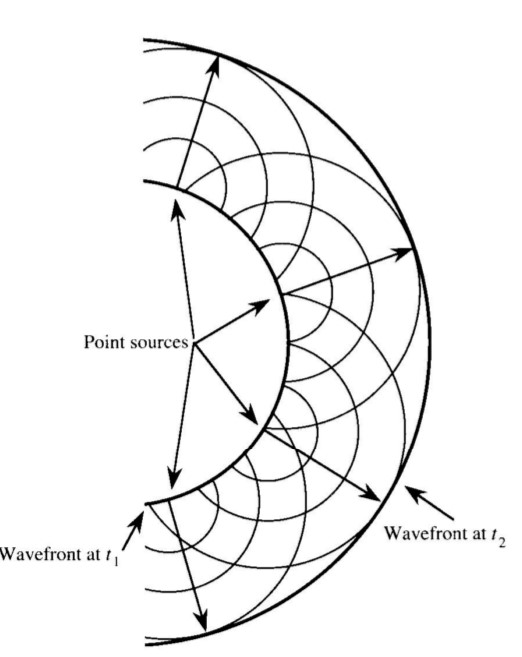
\includegraphics[height=0.5\textheight]{Images/huygens.jpg}
    \end{figure}
\end{frame}

\begin{frame}{Young's Double-Slit Experiment}
    \begin{figure}[htbp]
        \centering
        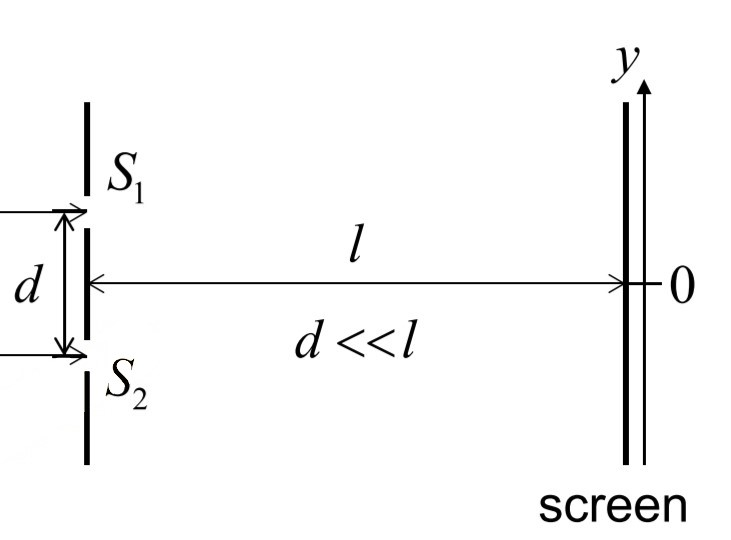
\includegraphics[height=0.5\textheight]{images/young.jpg}
        %\caption{}
        %\label{Fig:}
    \end{figure}

    If $d\ll l$, $\Delta \approx d\sin\theta \approx d \frac{y}{l}$.
    \begin{itemize}
        \item Constructive: $\Delta=m\lambda$
        \item Destructive: $\Delta= (2m+1)\lambda/2$
        \item $\abs{y_m} = m\lambda l/d$
    \end{itemize}
\end{frame}

\begin{frame}{Interference in Thin Films}
    \begin{beamerboxesrounded}[shadow=true]{Fresnel Equations}
        \begin{equation}
            E_{reflected} = \frac{n_1\cos\theta_{incident}-n_2\cos\theta_{reflected}}{n_1\cos\theta_{incident}+n_2\cos\theta_{reflected}} E_{incident}
        \end{equation}        
        Sign changes $\Rightarrow$ phase change by $\pi$ 
    \end{beamerboxesrounded}
    \vspace{.5em}
    Other examples:
    \begin{itemize}
        \item Soap bubbles, oil specks
        \item Inclined thin films
        \item Coatings: non-reflective, reflective
        \item Newton rings (circular)
    \end{itemize}
\end{frame}

%----------------------------------------------------------------------------------------
%	 Section 2
%----------------------------------------------------------------------------------------

\section{Exercise}

% \subsection{\bf Electric Field \& Gauss' Law}

% \begin{frame}{\bf Hw2 P2}
% A point charge $q$ is placed at the point $\mathbf{r}=0$.
% (a) By direct calculation show that the divergence of the 
% electric field $\operatorname{div} \mathbf{E}(\mathbf{r})=0$ 
% for all $\mathbf{r} \neq 0 .$ What can you say (qualitatively) 
% about the divergence at $\mathbf{r}=0 ?$
% (b) What is the condition $\operatorname{div} \mathbf{E}(\mathbf{r})$ 
% should satisfy at $\mathbf{r}=0$ for Gauss's law to be valid? 
% \end{frame}

% \begin{frame}{\bf Hw2 P9}
%     \begin{columns}
%         \begin{column}{.7\linewidth}
%             Two spherical cavities, of radii $r_{a}$ and $r_{b}$, are hollowed out from the interior of a neutral conducting ball of radius $R$. At the center of each cavity a point charge is placed: $q_{a}$ and $q_{b},$ respectively.
%             (a) Find the surface densities of charge $\sigma_{a}, \sigma_{b}$ on the walls of the cavities as well as on the surface of the ball $\sigma_{R}$.
%             (b) What is the electric field outside of the conductor?
%             (c) What is the electric field within each cavity?
%             (d) What is the force on $q_{a}$ and $q_{b} ?$
%             (e) Which of these answers would change if a third charge $q_{c}$ were brought near the conductor?

%         \end{column}
%         \begin{column}{.3\linewidth}
%             \begin{figure}
%                 \centering
%                 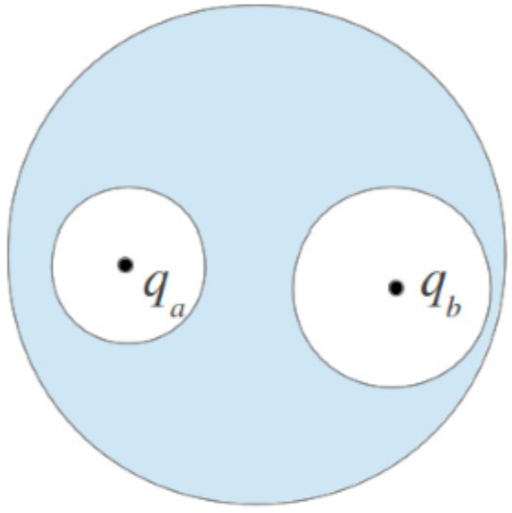
\includegraphics[scale=0.4]{images/ex2.png}
%             \end{figure}
%         \end{column}
%     \end{columns}

% \end{frame}

% \begin{frame}{\bf Hw3 P3}
%     What is the electric potential at a distance $s$ from an infinitely long straight wire charged with uniform density $\lambda$ ? Comment on your choice of the reference point.
% \end{frame}

% \begin{frame}{\bf Hw3 P4}
%     A conical surface (an empty ice-cream cone) carries a uniform surface charge with density $\sigma$. The height of the cone is $h,$ as is the radius of the top. Find the electric potential difference between points $\mathbf{r}_{A}$ (the vertex) and $\mathbf{r}_{B}$ (the center of the top).
% \end{frame}


% \begin{frame}{\bf Exercise 1}
% There are two positive point charges $q_1$ and $q_2$ locating at 
% $r_1$ and $r_2$ respectively. Now add a negative point charge $q_3$ 
% into the system. Please find out where it should be put and 
% what its magnitude is so that the electric forces exerted on 
% all three charges equal to 0.

% \begin{figure}[htbp]
%     \centering
%     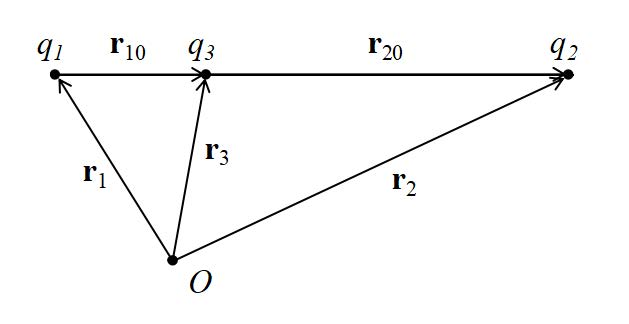
\includegraphics[scale = 0.8]{images/EF_1.jpg}
% \end{figure}
% \end{frame}


% \begin{frame}{\bf Exercise 2}
% There is a metal ball ($R$, $Q$) in space. Calculate the force between the upper and lower half balls.

% \begin{figure}[htbp]
%     \centering
%     \begin{tikzpicture}[scale=0.8]
%         \draw (0,0) circle (2);
%         \node[circle,fill = black!50,inner sep =2pt] () at (0,0) {};
%         \node[] () at (-0.5,0) {$Q$};
%         \node[] () at (1,0.5) {$R$};
%         \draw[->, line width = .035cm, black!80] (0,0) -- (1.42,1.42);
%     \end{tikzpicture}
% \end{figure}
% \end{frame}

% \subsection{\bf Electric Potential}

% \begin{frame}{\bf Hw3 P7}
%     Find the energy stored in a uniformly charged solid ball of radius $R$ and charge $q$. (This energy is also often called the "self-energy" of the charge distribution.) Do it in four different ways, using formulas we have derived in class:
% (a) Use $U_{\text {conf }}=\frac{1}{2} \int_{\Omega} \rho V d \tau$. \\
% (b) Use $U_{\text {conf }}=\frac{\varepsilon_{0}}{2} \int_{\text {all space }} E^{2} d \tau$. \\
% (c) Use $U_{\text {conf }}=\frac{\varepsilon_{0}}{2}\left(\int_{\Omega} E^{2} d \tau+\oint_{\Sigma} V \mathbf{E} \circ d \mathbf{A}\right)$ taking $\Sigma$ as a sphere of radius $a>R$ centered at the center of the ball. Comment on what happens as $a \rightarrow \infty$. \\
% (d) Find the amount of work needed to be done to assemble the ball by bringing infinitesimal charges from far away. 
% \end{frame}

% \begin{frame}{\bf Exercise 3}
%     \begin{columns}
%         \begin{column}{0.6\linewidth}
%         There are three point charges with mass \textit{m} and positive charge \textit{q}. Initially, they stay still 
%         at three vertexes of an equilateral triangle with side length \textit{l} and there is a rigid insulating rod connecting each 
%         point charge. Point \textit{C} is the center of the equilateral triangle. Now cut the rod between point charges 1 and 2, please find out:\\
%         (1) When point charge 3 reaches \textit{C}, what is its speed?\\
%         (2) During the entire process, what is the maximum speed of point charge 3?
%         \end{column}
%         \begin{column}{.4\linewidth}
%             \begin{figure}[H]
%                 \centering
%                 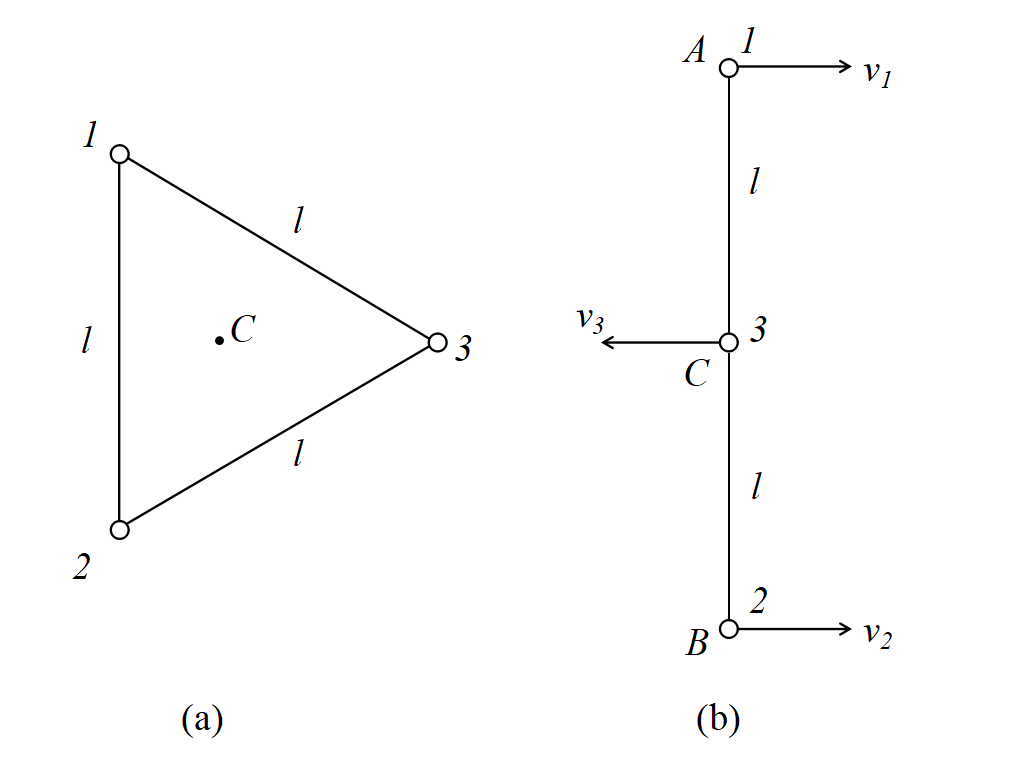
\includegraphics[scale=0.4]{images/009.png}
%                 \end{figure}
%         \end{column}
%     \end{columns}
% \end{frame}


% \begin{frame}{\bf Exercise 4}
%     Please first judge the following statement and then give your proof:\\
%     If a solid (means not hollow here) conductor carries a total charge of +\textit{Q} ($Q<0$), 
%     then the surface charge density $\sigma$ is greater than or equal to 0 everywhere on the surface of the conductor.
% \end{frame}

% %------------------------------------------------------%

% \subsection{\bf Method of Image}


% \begin{frame}{\bf Hw4 P5}

% (a) Calculate the electric potential in this region. 
% (b) What is the force on q? (c) How much work did it take to bring the charge q from infinity? 
% (d) For what particular angles does the method work?

% \begin{figure}
%     \centering
%     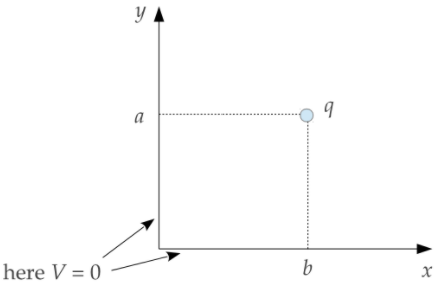
\includegraphics[scale=0.75]{images/ex5.png}
% \end{figure}

% \end{frame}


% \begin{frame}{\bf Exercise 5 (RC 2)}
%     There exists a point charge $Q$ and a conducting shell in space. The distance between the center of shell 
%     and the point charge is $a(a>R_0)$. Please find out the total amount of induced charge on the surface, in each case:
%     \begin{itemize}
%         \item The conducting shell is grounded
%         \item The conducting shell is neither grounded nor carrying any charge at first
%         \item The conducting shell is not grounded but at an electric potential $V_0$
%         \item The conducting shell is not grounded but carrying charge $q$ at first
%         \item What if $a<R_0$?
%     \end{itemize}
% \end{frame}

% %---------------------------------------------------%

% \subsection{\bf Capacitors}

% \begin{frame}{\bf Hw4 8}
%     Two square conducting plates with sides of length $L$ are separated by a distance $D$. A dielectric slab with relative permittivity $\varepsilon_{\mathrm{r}}$ and dimensions $L \times L \times D$ is inserted a distance $x$ into the space between the plates, as shown in the figure.
%     \begin{figure}
%         \centering
%         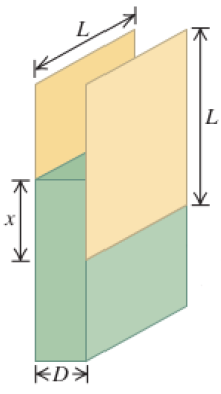
\includegraphics[scale=0.8]{images/HW4_8}
%     \end{figure}
% \end{frame}

% \begin{frame}{\bf Exercise 6}
%     Two metal boards are placed parallel to each other and 
%     separated at a distance $D=2cm$. The surface charge density 
%     on one board is $\sigma_{1}=3\mu C/m^2$ and $\sigma_{2}=6\mu C/m^2$ 
%     for another. A wax board with thickness $D/2$ whose relative 
%     permittivity is $\varepsilon_{r}=2$ is placed between two boards. 
%     Please find out the potential difference between two boards.
% \begin{figure}
%     \centering
%     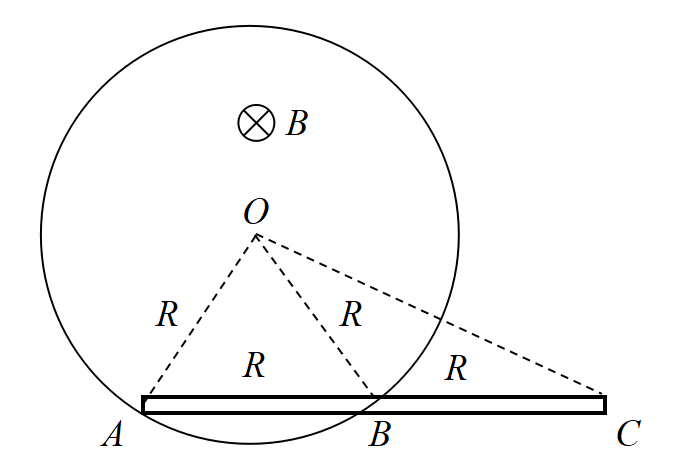
\includegraphics[scale=0.6]{images/013.png}
% \end{figure} 

% \end{frame}

% \begin{frame}{\bf Exercise 7}
% \begin{columns}
%     \begin{column}{.7\linewidth}
%         A parallel-plane capacitor is inserted into a beaker containing liquid dielectric with relative permittivity $\varepsilon_{r}$ and density $\rho$. 
%         Assume that the surface area of the plane is $S$ (with height $h$ and width $a$). The distance between two planes is $d$. There is an external power 
%         source to maintain the voltage across the capacitor at $V$. Given that the acceleration due to gravity is $g$, please find out the rise of liquid dielectric in the capacitor $h$.
%     \end{column}
%     \begin{column}{.3\linewidth}
%         \begin{figure}
%             \centering
%             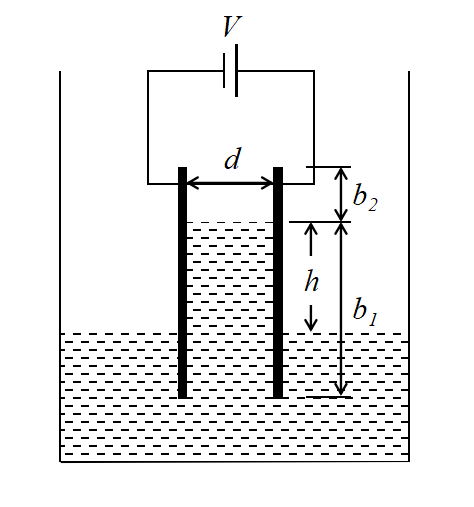
\includegraphics[scale=0.6]{images/014.png}
%         \end{figure}
%     \end{column}
% \end{columns}
% \end{frame}


% %-------------------------------------------%
% \subsection{\bf Electric Current}

% \begin{frame}{\bf Hw5 P1}
%     \begin{columns}
%         \begin{column}{.7\linewidth}
%             Two concentric spherical metal shells with radii $r_{a}, r_{b},$ 
%             where $r_{a}<r_{b},$ are separated by a weakly conducting material 
%             with conductivity $\sigma$. \\
%             (a) If they are maintained at potential difference $V,$ what current flows from one to each other? \\
%             (b) What is the resistance between the shells? \\ 
%             (c) Notice that if $r_{b} \gg r_{a},$ the outer radius $r_{b}$ is irrelevant. Determine the current flowing between two metal spheres, each of radius $r_{a}$, immersed deep in the sea and held quite far apart, if the potential difference between them is $V$.
%         \end{column}
%         \begin{column}{.3\linewidth}
%             \begin{figure}
%                 \centering
%                 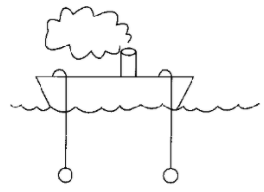
\includegraphics[scale=0.8]{images/HW5_1.png}
%             \end{figure}
%         \end{column}
%     \end{columns}
% \end{frame}

% \begin{frame}{\bf Hw5 P2}
%     Estimate the resistance between the wires.
%     \vspace{1em}
%     \begin{figure}
%         \centering 
%         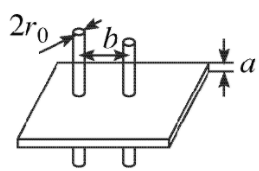
\includegraphics[scale = 1]{images/HW5_2.png}
%     \end{figure}
% \end{frame}


% \begin{frame}{\bf Exercise 8}
%     There are two concentric metal spheres with radius $a$ 
%     and $b$ respectively ($b>a$). There are materials with 
%     conductivity $\sigma=KE$ where $K$ is a positive constant 
%     and $E$ is the magnitude of the electric field. Now 
%     maintain the electric potential difference between 
%     two spheres at $V$, please find out the current flowing 
%     between two spheres.
% \end{frame}


% %---------------------------------------------%

% \subsection{\bf Magnetic Field}

% \begin{frame}{\bf Exercise 9}
%     A simple pendulum consists of a string with length $L$ 
%     and a ball carrying charge $+q$. The greatest swing angle is $\alpha$. 
%     In order to make this pendulum oscillate normally, what kind of restrict 
%     must be placed on the magnitude of the magnetic field?

%     \begin{figure}
%         \centering
%         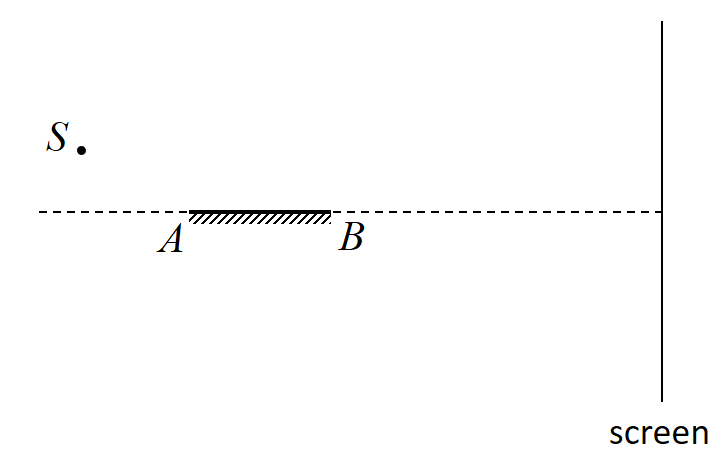
\includegraphics[scale=0.6]{images/005.png}
%     \end{figure}
% \end{frame}

% \begin{frame}{\bf Exercise 10}
%     There is a particle with mass m and charge $+q$ shot from point $a$ 
%     with a initial velocity $v_0$ pointing straightly towards point $b$. 
%     If the particle can exactly pass through point $b$, what are the possible 
%     values of the magnitude of $v_0$? (consider the gravitational force)

%     \begin{figure}
%         \centering 
%         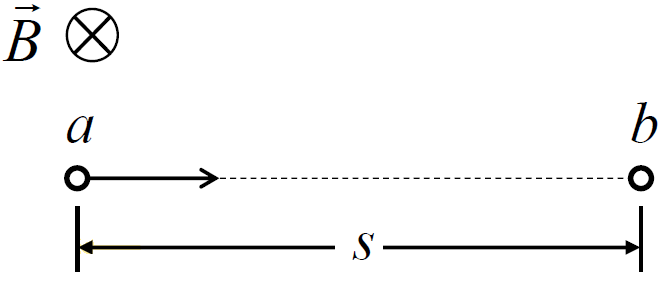
\includegraphics[scale=0.5]{images/Ex11.png}
%     \end{figure}
% \end{frame}


% %-----------------------------------------------%
% \subsection{\bf Ampere's Force}
% \begin{frame}{\bf Exercise 11}
%     $m_ab=5$g, $h=0.8$m, $L_ab=1$m, $C=400\mu$F, $\varepsilon=16$V, $B=0.5$T. 
%     The switch $S$ is first at position 1 for a long enough time, 
%     then suddenly moved to position 2. The metal bar will be 
%     catapulted to the ground and cover a horizontal distance 
%     $x=6.4$cm. Neglect the air drag and any friction, and given that the 
%     acceleration due to gravity $g=10$m/s$^{2}$, please 
%     find out the voltage across the capacitor after the 
%     metal bar is catapulted.

%     \begin{figure}[H]
%         \centering
%         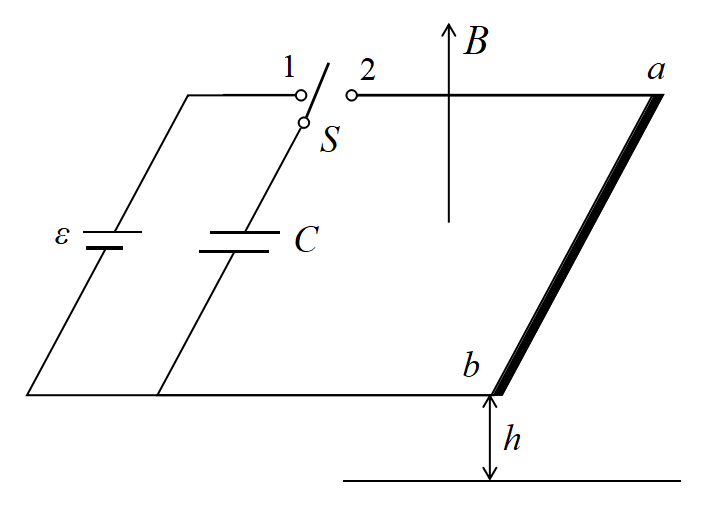
\includegraphics[scale=0.45]{images/007.png}
%     \end{figure}
% \end{frame}


%----------------------------------------------------------------------------------------
%	 CLOSING/SUPPLEMENTARY SLIDES
%----------------------------------------------------------------------------------------

\begin{frame}
    \begin{center}
        \LARGE\bf LALALA
    \end{center}

\end{frame}


\section*{Appendix}

%----------------------------------------------------------------------------------------

\begin{frame}{\bf References}
    \nocite{*} % Display all references regardless of if they were cited
    \bibliography{example.bib}
    \bibliographystyle{plain}
\end{frame}

\end{document}

